\chapter{Разработка сервиса}

\section{Формирование требований и ограничений к прототипу}

Анализ существующих технологий для проведения обмена активами между изолированными распределёнными реестрами с установлением доверия между сторонами, включая как прямой обмен, так и обмен с привлечением третьей стороны, выявил существенные проблемы, которые подрывают его эффективность и безопасность. Одним из ключевых аспектов остаётся проблема установления доверия между сторонами сделки и доверительной стороной. Для успешного проведения обмена активами, участники должны предоставить свои данные в соответствии с процедурой "Знай своего клиента" (KYC). Это требует больших усилий и времени для подтверждения подлинности предоставленных данных, что создаёт дополнительные задержки и неудобства. При этом доверительная сторона полагается на свою репутацию для обеспечения доверия между участниками. В то же время, практика показывает, что репутация не способна выступать полноценной гарантией надёжности таких сделок.

Проблемы безопасности представляется ещё одним существенным минусом. Доверительная сторона, которая играет роль посредника и хранителя данных, вероятно будет объектом кибератак. В случае успешного взлома злоумышленники получат доступ к конфиденциальной информации и активам участников сделки, что приводит к серьёзным финансовым потерям и утрате доверия к системе. Более того, доверительная сторона представляет собой единую точку отказа. Это означает, что она способна стать объектом давления со стороны регуляторов, что не исключает принудительных отказов от проведения сделок или даже блокировок активов. Такие случаи создают серьёзные риски для участников рынка, которые полагаются на бесперебойное функционирование доверительной стороны.

Все риски, связанные с деятельностью доверительной стороны, закладываются в комиссии за совершение обмена. Это приводит к увеличению издержек для участников сделки, делая обмен активами менее экономически выгодным. Высокие комиссии могут снизить привлекательность использования такой системы, особенно в условиях высокой конкуренции и наличия альтернативных решений. Использование доверительной стороны для обмена активами между изолированными блокчейнами не только увеличивает издержки, но и вносит дополнительные риски, связанные с безопасностью и регулированием. В результате, более предпочтительным способом обмена остаётся проведение сделок без установления доверия.

Обмен активами между изолированными распределёнными блокчейнами с использованием мостов, которые выпускают обёрнутые монеты, так же имеет свои недостатки. Один из главных минусов такой системы заключается в том, что процесс оборачивания активов не является полноценным обменом. Вместо реального перемещения активов между реестрами, создаются обёрнутые монеты, представляющие собой токены, обеспеченные оригинальными активами. Это порождает вопросы относительно надежности и безопасности таких токенов, поскольку они зависят от корректного хранения и управления залогом.

Вопрос о том, кто и как контролирует залог, приобретает первостепенное значение. Это хранение обязательно должно быть описано в смарт-контракте, чтобы минимизировать риски, связанные с доверием к человеческому фактору. Если система хранения залога не является достаточно прозрачной и надёжной, то мы снова приходим к проблеме доверия, о которой говорили выше. Ещё один момент, где может возникнуть вопрос к доверию, это среда исполнения моста: мосты должны быть децентрализованными. Это, в свою очередь, добавляет ещё больше сложности в разработку и поддержку таких систем.

Кроме того, схема использования мостов для обмена активами достаточно сложна в разработке и поддержке, т.к. требует привлечения оракулов. Оракулы необходимы для обеспечения корректного функционирования смарт-контрактов, предоставляя им достоверные внешние данные. Однако использование оракулов влечет за собой дополнительные затраты на разработку и поддержку этой инфраструктуры. Пользователи вынуждены оплачивать эти затраты через комиссии за сделки, что увеличивает общие издержки и снижает экономическую эффективность системы.

Обмен активами между блокчейнами с использованием мостов, функционирующих через пулы ликвидности, так же не способен решить все существующие проблемы. Главое ограничение данной системы кроется в том, что ее эффективность напрямую зависит от наличия достаточного объема торгов по популярным торговым парам с высокой ликвидностью. Эти мосты эффективно работают только при наличии достаточного объёма ликвидности, что ограничивает их применение к менее популярным активам. В результате, пользователи, желающие обменять редкие или новые активы, могут столкнуться с проблемами, такими как "проскальзывание цены". Проскальзывание возникает, когда фактическая цена сделки отличается от ожидаемой из-за изменений в спросе и предложении в пуле ликвидности. Это ведёт к неопределённости для участников обмена, так как они не могут быть уверены в конечной цене сделки.

Поставщики ликвидности, участвующие в пулах, получают процент от каждой сделки, который оплачивается сторонами процесса обмена. Эти комиссии могут существенно увеличить общие издержки участников сделки, особенно если ликвидность в пуле низкая. Фактически, пользователи вынуждены учитывать не только комиссии за транзакции в самих блокчейнах, но и дополнительные издержки на оплату поставщиков ликвидности.

Если говорить об обмен активами между блокчейнами с использованием релейных блокчейнов, то ключевым минусом этого подхода остаётся требование, чтобы все блокчейны принадлежали одной экосистеме. Это условие существенно ограничивает возможность интеграции блокчейнов с большой историей и широким сообществом пользователей, таких как Bitcoin и Ethereum.

Централизация релейных блокчейнов также вызывает серьёзные вопросы доверия. Это традиционные риски, связанные с возможностью единой точки отказа и злоупотребления полномочиями.

Механика атомарных свапов с использованием Hash Time-Locked Contracts (HTLC) является одним из наиболее эффективных и безопасных методов для обмена активами между блокчейнами из рассмотренных нами. Использование этого подхода гарантирует полное отсутствие необходимости доверия между сторонами сделки. Все гарантии обеспечиваются самой механикой свапов, что исключает потребность в доверительных отношениях или третьих сторонах, минимизируя тем самым риски мошенничества и недобросовестного поведения.

Отсутствие регуляторных рисков оказывается ещё одним существенным преимуществом атомарных свапов. Поскольку в сделке участвуют только две стороны, нет необходимости вовлекать центральные или регуляторные органы. Это упрощает процесс и снижает вероятность внешнего вмешательства. Особенно важно это в контексте международных обменов, где регуляторные требования могут ощутимо различаться и создавать дополнительные сложности для участников сделки.

Фиксированная цена и отсутствие дополнительных комиссий делают атомарные свапы экономически привлекательным вариантом для обмена активами. Участники сделки заранее согласовывают цену обмена, что исключает вероятность проскальзывания или непредвиденных расходов. Пользователи могут точно прогнозировать затраты и результаты сделки, даже в условиях волатильных рынков.

Безопасность участников обеспечивается встроенными механизмами HTLC. В случае возникновения проблем, таких как непреднамеренные ошибки или отказ одной из сторон от завершения сделки, балансы автоматически возвращаются в исходное состояние. Ни одна из сторон не понесёт убытки, если сделка не будет завершена в соответствии с заранее оговоренными условиями. Такой уровень безопасности делает атомарные свапы предпочтительным выбором для пользователей, стремящихся минимизировать риски.

Дополнительным плюсом служит то, что существующие блокчейны можно модифицировать для поддержки HTLC. Если блокчейн изначально не поддерживает требуемые технологии, такие как алгоритм SHA256, их можно добавить в блокчейн. Это расширяет применимость атомарных свапов и позволяет интегрировать их в различные блокчейн-системы, улучшая их функциональность и интероперабельность. Так, в сети BitShares первая реализация HTLC была представлена только в третьей версии блокчейна\cite{label28}.

Механика атомарных свапов с использованием HTLC представляет собой надёжный и эффективный метод обмена активами между блокчейнами. Полное отсутствие необходимости в доверии между сторонами, отсутствие регуляторных рисков, фиксированная цена без дополнительных комиссий, высокая безопасность для участников и возможность адаптации существующих блокчейнов делают этот подход предпочтительным для широкого круга пользователей. Эти преимущества обеспечивают высокую надёжность и экономическую эффективность обменов, способствуя развитию децентрализованных финансовых систем и укреплению доверия к блокчейн-технологиям.

\subsection{Решаемые задачи}

Разработка сервиса для проведения обмена активами между изолированными распределёнными реестрами без установления доверия требует решения следующих задач:

\begin{enumerate}
\item Создание сервиса, который будет управлять действиями пользователя в процессе обмена активами:
	\begin{enumerate}[label*=\arabic*.]
	\item Инициализация контракта.\\
	Реализовать функцию инициализации контракта с указанием суммы активов для обмена и времени блокировки.
	\item Управление ключами контракта.\\
	Обеспечить возможность получения ключа контракта от пользователя либо генерации криптостойкого ключа на стороне сервиса.
	\item Мониторинг и отображение статуса.\\
	Внедрить механизм отображения статуса операции и мониторинга блокчейна на предмет обновлений.
	\item Отправка транзакций.\\
	Реализовать отправку транзакций в блокчейн с использованием предоставленных ключей контракта и параметров.
	\end{enumerate}
\item Подключение к сервису блокчейна, способного исполнять смарт-контракты в виртуальной машине:
	\begin{enumerate}[label*=\arabic*.]
	\item Разработка смарт-контракта.\\
	Создать смарт-контракт, обеспечивающие функциональность.
	\item Интеграция смарт-контракта с сервисом.\\
	Внедрить поддержку взаимодействия сервиса с разработанным смарт-контрактом, обеспечивая управление и выполнение условий HTLC.
	\end{enumerate}
\item Подключение к сервису блокчейна, не обладающего виртуальной машиной, но выполняющего требования для HTLC:
	\begin{enumerate}[label*=\arabic*.]
	\item Интеграция с API блокчейна.\\
	Реализовать взаимодействие сервиса с API блокчейна для управления HTLC, обеспечивая все необходимые операции для создания, мониторинга и завершения HTLC.
	\end{enumerate}
\item Обеспечение доверия:
	\begin{enumerate}[label*=\arabic*.]
	\item Полная децентрализация.\\
	Гарантировать, что использование сервиса не требует доверия между сторонами или к третьей стороне. Это означает, что каждая сторона может запустить экземпляр сервиса самостоятельно, без необходимости использования централизованного сервера или облачной базы данных.
	\end{enumerate}
\end{enumerate}

Эти задачи должны быть выполнены с соблюдением существующих лучших практик в области разработки реальных блокчейнов. Учитывая, что это прототип, допускается вывод подробнейшей отладочной информации.


\section{Описание бизнес-логики и архитектура решения}

\subsection{Выбор технологий для разработки}

Для создания сервиса обмена активами между изолированными блокчейнами с использованием механизма атомарных свапов через HTLC, были выбраны Ethereum, BitShares и React. Эти технологии обладают уникальным характеристикам и преимуществам, которые вместе обеспечивают надежность, эффективность и удобство использования сервиса.

Ethereum завоевал репутацию одной из самых популярных и функциональных блокчейн-проектов. Его широкое распространение и поддержка огромного количества токенов стандарта ERC-20 делают его идеальной платформой для обмена различными активами. Ethereum обладает широкими возможностями для разработки смарт-контрактов, что позволяет реализовывать такие сложные механизмы, как HTLC. Смарт-контракты в Ethereum обладают высокой гибкостью и позволяют устанавливать условия для атомарных свапов, такие как условное хранение активов, проверка хэшей и установление таймаутов. Кроме того, большое и активное сообщество разработчиков Ethereum накопило заметный опыт лучших практик и предоставляет доступ к множеству примеров, библиотек и решений, что заметно облегчает процесс разработки.

BitЫhares был выбран благодаря своей высокой производительности и низким комиссиям, которые достигаются за счет использования консенсусного алгоритма DPoS (Delegated Proof of Stake). Это делает Bitshares привлекательным для быстрого и недорогого обмена активами. Bitshares разработан с акцентом на децентрализованные обмены активов внутри сети, что даёт встроенную поддержку обмена активами и высокую ликвидность. Возможность торговать различными активами, включая криптовалюты и токенизированные активы, делает Bitshares интересной платформой для проведения обмена.

React был выбран для создания пользовательского интерфейса благодаря своей гибкости и высокой производительности. Это мощная JavaScript-библиотека, которая позволяет разрабатывать динамичные и отзывчивые веб-приложения. Широкая экосистема и поддержка React ускоряют процесс разработки благодаря большому количеству готовых компонентов, библиотек и инструментов. Более того, React легко интегрируется с различными блокчейн-платформами через библиотеки, такие как web3.js для Ethereum и bitsharesjs для Bitshares. Это позволяет создать единый интерфейс для взаимодействия с различными блокчейн-сетями, обеспечивая удобство и простоту использования для конечных пользователей. Кроме того, исследователи отмечают, что JavaScript выходит на ведущее место среди языков, используемых для исследования в области цифровых валют\cite{label29}.

Дополнительно, React-приложение упаковано в Docker-контейнер, что предоставляет ряд весомых преимуществ для разработки, развёртывания и эксплуатации сервиса. Упаковка React-приложения в Docker-контейнер делает возможным высокую портативность решения. Контейнеры Docker включают все необходимые зависимости и окружение для работы приложения, обеспечивая гарантии корректную окружения на любых машинах, независимо от их конфигурации. В нашем случае, использование Docker даёт сторонам сделки простой способ запустить экземпляр нашего сервиса на своей инфраструктуре, так что нет необходимости доверять даже облачным провайдерам.

В нашем решении React-приложение отвечает за подготовку транзакций, которые затем должны быть подписаны и отправлены с использованием совместимого с Ethereum кошелька. Этот подход обеспечивает безопасность и контроль над приватными ключами, поскольку они никогда не покидают пользовательское устройство. Мы протестировали наше решение с популярными кошельками Metamask и Enkrypt(MyEtherWallet). Metamask, являясь одним из самых популярных Ethereum-кошельков, предоставляет удобный интерфейс для взаимодействия с dApp и предоставляет безопасное хранение ключей. Он интегрируется как расширение браузера, что упрощает использование и повышает доступность для пользователей. Enkrypt(MyEtherWallet) предоставляет богатый функционал и высокий уровень безопасности, позволяя пользователям управлять своими активами через веб-интерфейс.

Поскольку API для взаимодействия с Ethereum-кошельками стабильно и широко распространено, мы уверены, что наше приложение будет совместимо и с другими кошельками, включая аппаратные. Аппаратные кошельки, такие как Ledger и Trezor, обеспечивают дополнительный уровень безопасности, изолируя приватные ключи от не доверенной среды. Кроме аппаратных кошельков, многие мобильные и десктопные Ethereum-кошельки поддерживают необходимый функционал для подписания и отправки транзакций, подготовленных нашим React-сервисом.

В нашем решении не требуется использовать традиционную базу данных, поскольку блокчейн сам по себе представляет собой огромную распределённую базу данных. Блокчейн, будь то Ethereum или Bitshares, хранит все данные транзакций и состояния активов в распределённой и неизменяемой форме. Использование блокчейна в качестве базы данных устраняет необходимость в централизованном хранении и управлении данными. В нашем случае, обмен активами между пользователями происходит напрямую через блокчейн, Это значит, что мы всегда может использовать API чтобы найти нужную операцию и узнать её статус.

Использование Ethereum и Bitshares для реализации сервиса атомарных свапов позволяет сочетать преимущества обеих платформ: гибкость и мощность смарт-контрактов Ethereum с высокой производительностью и встроенными механизмами децентрализованного обмена Bitshares. React, в свою очередь, обеспечивает создание удобного и отзывчивого интерфейса, который легко интегрируется с обеими блокчейн-платформами. Вместе эти технологии позволяют создать крайне надежный и эффективный сервис для обмена активами между изолированными распределёнными реестрами без необходимости установления доверия между сторонами.

\subsection{Структура сервиса}

Структурно сервис представляет из себя смарт-контракт и веб-интерфейс. Схема сервиса представлена на рис. \ref{pic:architecture}.

\begin{figure}[H]
\centering
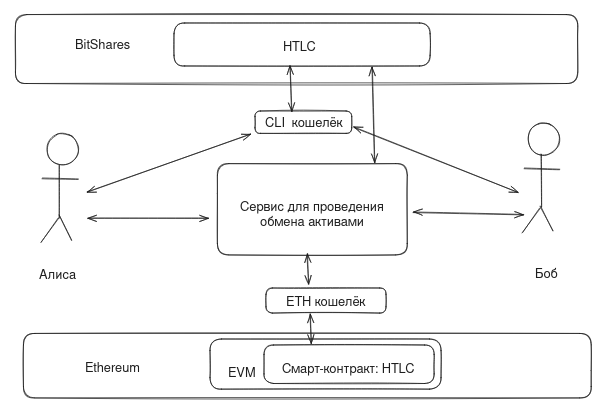
\includegraphics[scale=0.65]{res/architecture}
\caption{Структура сервиса}
\label{pic:architecture}
\end{figure}

На этой схеме изображёны участники обмена активами, Алиса и Боб, с и две изолированные блокчейн сети -- BitShares и Ethereum. Так же на схеме показаны два основных элемента, которые входят в наш сервис -- это смарт-контракт для сети Ethereum и веб-интерфейс сервиса, который обеспечивает безопасный обмен.

В верхней части диаграммы находится платформа BitShares, где HTLC реализован как часть узла блокчейна. Алиса и Боб взаимодействуют с BitShares через CLI кошелёк, который служит интерфейсом для выполнения операций. С этого кошелька уходят подписанные операции в сеть BitShares. Из соображений безопасности, мы не стали хранить приватный ключ пользователя в сервисе. Это, очевидно, снижает удобство всей операции, но тут мы сталкиваемся с классической проблемой выбора между удобством и безопасностью.

Сервис для проведения обмена активами генерирует команды для CLI кошелька на стороне BitShares, и готовит транзакции на подписание любым ETH кошельком на стороне Ethereum. Этот сервис получает команды от Алисы и Боба, обрабатывает их и отслеживает состояние контрактов в обеих блокчейнах.

На стороне Ethereum изображён EVM (Ethereum Virtual Machine) и смарт-контракт HTLC, который аналогично HTLC на BitShares обеспечивает процесс обмена активами без доверия. Обе стороны сделки имеют возможность провести валидацию содержимого блокчейна, чтобы удостовериться что он выполняет ровно то, что заявлено..

Сам сервис, CLI кошелёк для BitShares и ETH кошелёк для Ethereum изображены в одном экземпляре, но это сделано только чтобы не загромождать схему. На самом деле, каждый пользователь пользуется своим экземпляром.

Диаграмма иллюстрирует, как Алиса и Боб, используя свои кошельки и взаимодействуя через сервис для проведения обмена активами, могут безопасно обмениваться активами между двумя различными блокчейн-платформами, BitShares и Ethereum, с использованием механизма HTLC для обеспечения безопасности и надежности процесса.

\subsection{Алгоритм работы сервиса}

Упрощенный алгоритм работы сервиса представлен на диаграмме последовательности на рис. \ref{pic:sequence}. В декомпозиции этого процесса сложность представляет определение границ каждой сущности, чтобы привести работу обоих блокчейнов к единой точке отсчёта.

\begin{figure}[H]
\centering
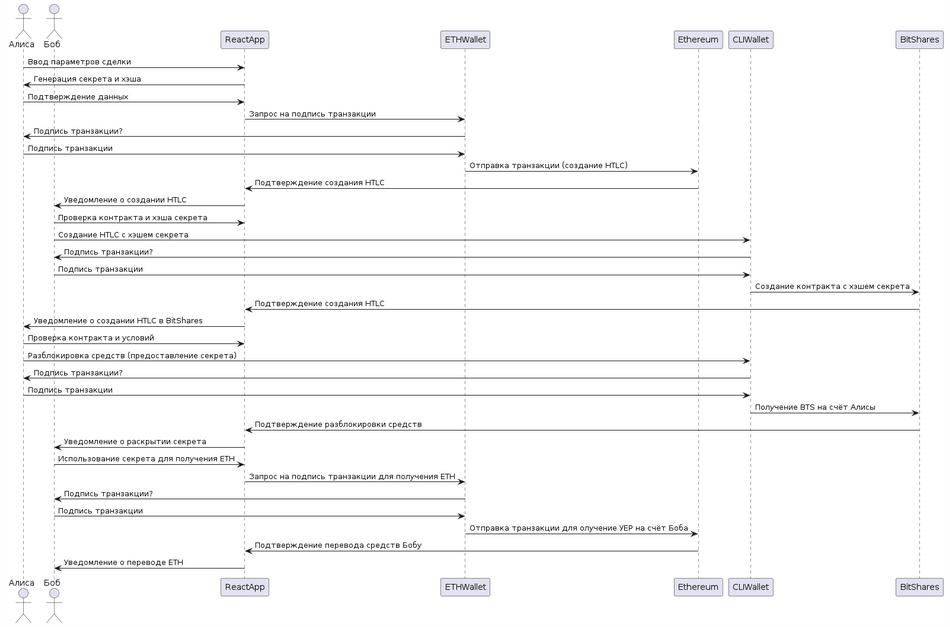
\includegraphics[scale=0.5]{res/sequence}
\caption{Алгоритм работы сервиса на диаграмме последовательности}
\label{pic:sequence}
\end{figure}

Алиса и Боб договорились провести обмен активами: Алиса отдаёт свои ETH, а в ответ получает BTS от Боба. Первым шагом Алиса запускает наше React приложение, где она вводит параметры предстоящей сделки. В интерфейсе она указывает максимальное время исполнения заявки, сумму ETH для обмена и адрес получателя, которым будет Боб. Кроме того, приложение генерирует уникальный секрет и вычисляет его хэш, который затем используется в транзакции. После подготовки всех данных приложение вызывает Enkrypt (MyEtherWallet) для подписания этой транзакции. Алиса подписывает и отправляет транзакцию в сеть Ethereum, где создаётся HTLC контракт.

Когда транзакция проходит в Ethereum, Боб получает уведомление о появлении нового HTLC контракта. Он проверяет, что контракт создан на его адрес, и сверяет хэш секрета. После этого Боб создаёт аналогичный HTLC контракт в сети BitShares с помощью CLI-кошелька. В этом контракте получателем указывается адрес Алисы, а хэш совпадает с тем, что он увидел в сети Ethereum. Существенной особенностью процесса является то, что время жизни контракта в BitShares должно быть меньше, чем в Ethereum, чтобы минимизировать риски для Боба. Если Алиса не сможет предоставить секрет вовремя, Боб сможет вернуть свои BTS.

После создания контракта в сети BitShares, Алиса получает уведомление и проверяет условия контракта, включая количество BTS и параметры хэш-замка. Убедившись в правильности всех условий, Алиса использует свой CLI-кошелёк, чтобы предоставить секрет и получить свои BTS. Поскольку контракт был создан с использованием известного хэша секрета, Алиса легко разблокирует средства и забирает их.

Как только Боб видит, что секрет был раскрыт в сети BitShares, он использует этот же секрет для получения своих ETH из контракта в сети Ethereum. Сервис помогает ему подготовить соответствующую транзакцию, и Боб подписывает её с помощью Enkrypt (MyEtherWallet). Остальные пользователи могут видеть раскрытый секрет, но ничего не могут сделать с активами, так как контракт чётко определяет, что только Боб может забрать ETH.

Сервис обеспечивает безопасный обмен активами между изолированными распределёнными реестрами с использованием механизма атомарных свопов через HTLC. Реализация на React обеспечивает удобный интерфейс для взаимодействия пользователей с блокчейнами, а использование Enkrypt (MyEtherWallet) и CLI BitShares позволяет надёжно подписывать и отправлять транзакции. Этот подход позволяет избежать необходимости доверия между сторонами и минимизирует риски благодаря использованию проверенных криптографических методов и смарт-контрактов.

\section{Программная реализация прототипа}

\subsection{Сервис обмена}

Сервис обмена представляет собой графическое приложение на React. Приложение упаковано в Docker, это значит что любая сторона может запустить экземпляр приложения независимо друг от друга. Но даже если будет использоваться один веб-сервер для раздачи JS-файлов, они всё равно могут быть проверены сторонами перед исполнением.

Для взаимодействия с Ethereum, используется универсальное API, которое позволяет подписывать транзакции в отдельном окне. BitShares не имеет интеграции с такими средствами, а хранить приватный ключ в браузере мы сочли недостаточно надёжным. Поэтому для BitShares мы даём команды, которые пользователь может выполнить в cli-интерфейсе.

Листинг \ref{lst:app} представляет собой исходный код основной формы React-приложения для реализации интерфейса для атомарного свопа между Ethereum (ETH) и BitShares (BTS).

\lstinputlisting[language=JavaScript, caption={React приложение атомарного свапа}, captionpos=t, label=lst:app]
{res/App.js}

В данном коде, начиная с первой строки, происходит импорт необходимых зависимостей из библиотек \textit{react} и \textit{styled-components}, а также компонентов из локальных файлов (строки 1-5). Далее создается стилизованный компонент \textit{Container}, который устанавливает базовые стили для всего приложения, такие как цвет фона, минимальная высота и параметры выравнивания (строки 8-16). Компонент \textit{Header} стилизует заголовок, задавая ему цвет и отступы (строки 18-21).

Затем определяется контейнер для вкладок (\textit{TabContainer}), который используется для выравнивания элементов вкладок (строки 23-26). Сами вкладки (\textit{Tab}) стилизованы с учетом состояния \textit{active}, определяющего их фон и другие параметры стиля, такие как отступы, границы и эффекты при наведении (строки 28-41). Компонент \textit{Content} задает стили для основного содержимого, включая белый фон, отступы, скругленные углы и тень (строки 43-49).

Функция \textit{App} представляет собой основной функциональный компонент приложения. В нем используется хук \textit{useState} для управления активной вкладкой, которая по умолчанию установлена на \textit{'eth'} (строка 53). Если в браузере пользователя не установлен MetaMask, выводится предупреждение и выполнение функции прекращается (строки 45-58). Определяются провайдер Ethereum и адрес контракта, а также провайдер BitShares (строка 62).

Основной JSX-возврат начинается с рендеринга контейнера \textit{Container}, в который вложены заголовок (\textit{Header}), контейнер вкладок (\textit{TabContainer}) и основной блок содержимого (\textit{Content}) (строки 65-96). В \textit{TabContainer} размещаются две вкладки, одна для Ethereum, другая для BitShares, при клике на которые активная вкладка изменяется с помощью функции \textit{setActiveTab} (строки 79-94). 

Содержимое блока \textit{Content} меняется в зависимости от активной вкладки. Если активна вкладка \textit{eth}, отображаются компоненты \textit{InitiateSwap}, \textit{Withdraw}, \textit{CheckStatus} и \textit{Refund}, которым передаются необходимые параметры (строки 73-78). Если активна вкладка \textit{bts}, показывается статический контент с инструкциями для BitShares и компонент \textit{CheckStatus} (строки 81-93).

В конце файл экспортирует компонент \textit{App} по умолчанию, чтобы его можно было использовать в других частях приложения (строка 100).

Рассмотрим ещё один пример кода -- компонент инициализации HTLC в листинге \ref{lst:InitiateSwap}.

\lstinputlisting[language=JavaScript, caption={Фукциональный React-компонент инициализации атомарного свапа}, captionpos=t, label=lst:InitiateSwap]
{res/InitiateSwap.js}

В этом коде сначала импортируются необходимые зависимости из библиотек \textit{react} и \textit{styled-components}, а также модуль \textit{ethers} из библиотеки \textit{ethers.js} для работы с Ethereum (строки 1-3). Затем определяются стили для компонента \textit{input} в объекте \textit{styles}, который включает отступы, размер шрифта, скругленные углы и границу (строки 5-12).

Создается стилизованный компонент \textit{Form}, который представляет собой контейнер для формы, выстраивающий свои элементы в колонку с промежутком в 10 пикселей (строки 15-19). Компонент \textit{Input} стилизует поля ввода, добавляя отступы, границу и скругленные углы (строки 21-25). Кнопка \textit{Button} имеет стили для фона, цвета текста, отступов, скругленных углов и эффекта при наведении (строки 27-38). Компонент \textit{Message} отображает сообщение, изменяя его цвет в зависимости от свойства \textit{error} (строки 40-43).

Компонент \textit{InitiateSwap} является функциональным компонентом, который принимает параметры \textit{ethContractAddress}, \textit{ethProvider} и \textit{btsProvider} (строка 45). Внутри него используются хуки \textit{useState} для управления состоянием различных полей формы, таких как получатель ETH, сумма ETH, секрет, время блокировки и сообщение, а также для проверки валидности адреса получателя (строки 46-51).

Функция \textit{generateSecret} создает новый секрет с помощью \textit{ethers.hexlify} и \textit{ethers.randomBytes}, и устанавливает его в состоянии компонента (строки 53-61). Функция \textit{validateRecipient} проверяет валидность Ethereum-адреса с помощью \textit{ethers.isAddress} (строки 58-61). В функции \textit{handleRecipientChange} обрабатывается изменение адреса получателя, обновляя состояние и проверяя валидность адреса (строки 63-67).

Основная функция \textit{initiateSwap} выполняет процесс инициирования свопа. Она запрашивает аккаунты у пользователя, создаёт контракт, инициирует своп, обрабатывает транзакцию и отображает сообщение о результате (строки 69-90). 

JSX-возврат компонента \textit{InitiateSwap} включает форму с заголовком и полями ввода для получателя ETH, суммы ETH, секрета и времени блокировки, а также кнопки для генерации секрета и инициирования свопа. Поле ввода для получателя ETH динамически меняет стили в зависимости от его валидности (строки 92-130).

Компонент \textit{InitiateSwap} экспортируется по умолчанию для использования в других частях приложения (строка 132).

Проект состоит из множества других компонентов и служебных файлов (Dockerfile, docker-compose.yml), но их подробное рассмотрение нецелесообразно.

С точки зрения анализа лучших практик, можно отметить предупреждения от системы сборки React-проекта об устаревании некоторых пакетов, которые используются в качестве зависимости. Это не является критической проблемой, т.к. сервис может работать локально и не имеет доступа к приватным ключам пользователя. С точки зрения UI/UX можно поработать над более наглядным интерфейсом, добавлением динамики при обработке транзакции узлами блокчейнов и сделать более подробные инструкции для BitShares части проекта. Но эти исследования достаточно ресурсоёмки, и останутся за пределами данной работы.

\subsection{Интеграция блокчейна с виртуальной машиной (Ethereum)}

\subsubsection{Смарт-контракт для блокчейна Ethereum}

Для исполнения HTLC в блокчейне Ethereum был подготовлен специальный смарт-контракт на языке Solidity (см. листинг \ref{lst:solidity}). Этот смарт-контракт реализует механизм атомарных свапов (Atomic Swap) с использованием Hash Time-Locked Contracts (HTLC) на языке Solidity.

\lstinputlisting[language=Solidity, caption={Фрагмент исходного кода модифицированного файла игры}, captionpos=t, label=lst:solidity]
{res/HTLC.sol}

\subsubsection{Описание смарт-контракта и анализ лучших практик}

Рассмотрим содержимое этого смарт-контракта:

В строках 1-2 объявлена лицензия MIT. Это разрешающая лицензия, которая позволяет использовать, модифицировать и распространять код при условии сохранения оригинального уведомления о лицензии. Так же указана версия компилятора Solidity 0.8.0.
   
В строке 20 начинается объявление смарт-контракта под названием \textit{AtomicSwap}, который реализует хешированные контракты с временной блокировкой для обмена ETH.

В строке 22 объявлена структура \textit{Swap}, которая содержит информацию о каждом обмене. Структура включает поля: 
\begin{itemize}
\item отправитель;
\item получатель;
\item сумма перевода;
\item хеш секретного ключа;
\item срок блокировки;
\item флаги состояния исполнения и возврата средств;
\item сам секретный ключ (пока ключ не раскрыт, это поле будет пустым).
\end{itemize}

В строке 34 объявлено хранилище \textit{swaps}, представляющее собой отображение идентификатора свопа (\textit{bytes32}) на структуру \textit{Swap}. Это позволяет сохранять и получать данные о каждом свопе по его уникальному идентификатору.

В строках 37-49 объявлены события \textit{SwapInitiated}, \textit{Withdraw} и \textit{Refund}, которые логируют важные действия в контракте: создание нового свопа, вывод средств и возврат средств соответственно.

В строках 60-97 реализована функция \textit{initiateSwap}, которая создаёт новый своп. Эта функция принимает адрес получателя, хеш секретного ключа и срок блокировки, а также сумму ETH через \textit{msg.value}. В функции проверяются условия корректности входных данных и создаётся уникальный идентификатор свопа. Затем данные свопа сохраняются в хранилище, и генерируется событие \textit{SwapInitiated}.

В строках 105-121 реализована функция \textit{withdraw}, которая позволяет получателю вывести ETH, зная секретный ключ. Функция проверяет корректность свопа, соответствие хеша секретного ключа, текущее время и статус свопа. Если все условия выполнены, средства переводятся на адрес получателя, и генерируется событие \textit{Withdraw}.

В строках 128-140 реализована функция \textit{refund}, которая позволяет отправителю вернуть свои средства после истечения срока блокировки. Функция проверяет существование свопа, права отправителя, срок блокировки и статус возврата. При выполнении условий средства возвращаются отправителю, и генерируется событие \textit{Refund}.

В строках 148-150 реализована функция \textit{getSecretHash}, которая позволяет получить хеш секретного ключа для указанного свопа. Эта функция публичная и предназначена для получения информации о свопе.

В строках 158-161 реализована функция \textit{getSecret}, которая позволяет получить секретный ключ для указанного свопа после его успешного завершения (вывода средств). Эта функция также публичная, но доступ к секрету возможен только после успешного завершения свопа.

С точки зрения следования лучшим практикам, использование \textit{block.timestamp} может быть ненадежным, так как майнеры могут слегка манипулировать этим значением. Хотя это не является критическим для нашего случая, это требование может варьироваться в зависимости от потребностей и сценариев использования. Текущая реализация позволяет только получателю снять средства или инициатору вернуть их после истечения временного замка. В некоторых случаях может быть полезно предусмотреть возможность для инициатора свапа отозвать средства до истечения временного замка, если это необходимо. Контракт не допускает повторную инициацию свапа с тем же \textit{\_swapId}. Теоретически существует вероятность, что в следствии коллизии разные входные данные могут дать одно и тоже значение на выходе в следствии коллизии хэш-функции. Переменные состояния, такие как \textit{withdrawn} и \textit{refunded}, могут быть объединены в один байт с битовыми флагами, что уменьшит потребление газа, но сделает код менее читаемым.

Представленный смарт-контракт полностью справляется с задачей обеспечения безопасного выполнение атомарных свапов. Использованием временных замков и хешей секретных ключей надёжно защищает интересы сторон обмена.

\subsubsection{Процесс выполнения смарт-контракта}

Виртуальная машина Ethereum (EVM) представляет собой децентрализованную вычислительную платформу, на которой выполняются смарт-контракты, написанные на языке программирования Solidity. Когда смарт-контракт, такой как описанный выше, загружается в блокчейн Ethereum, он компилируется в байт-код, который может быть интерпретирован и выполнен EVM.

Процесс выполнения смарт-контракта EVM начинается с транзакции, инициированной пользователем или другим контрактом. Транзакция включает данные, такие как адрес контракта, который будет вызван, и передаваемые параметры. В случае представленного выше смарт-контракта, первая транзакция может быть вызовом функции \textit{initiateSwap}, которая инициализирует новый своп.

Когда транзакция достигает узла в сети Ethereum, узел передает транзакцию EVM для обработки. EVM создает изолированное окружение для выполнения кода контракта, обеспечивая, что каждое выполнение является детерминированным и не зависит от состояния других контрактов. Это окружение включает стек, область памяти и область хранения, которые используются для управления данными и состоянием контракта.

EVM начинает выполнение байт-кода контракта, интерпретируя каждую инструкцию последовательно. В функции \textit{initiateSwap}, EVM выполняет проверки условий, таких как корректность адреса получателя и положительное значение \textit{msg.value}, чтобы убедиться в валидности данных. Затем EVM генерирует уникальный идентификатор свопа, используя хеширование, и сохраняет данные свопа в области хранения контракта. После успешного выполнения этих операций, EVM создает лог-событие \textit{SwapInitiated}, записывая его в журнал транзакций, что позволяет участникам сети отслеживать произошедшие изменения.

Аналогичным образом, при вызове функции \textit{withdraw} или \textit{refund}, EVM выполняет последовательность инструкций, соответствующих этим функциям. Для \textit{withdraw}, EVM проверяет, что секретный ключ соответствует хешу и что срок блокировки не истек. Если все условия выполняются, средства переводятся получателю, и статус свопа обновляется. В случае \textit{refund}, EVM проверяет, что срок блокировки истек и что своп не был уже возвращен, после чего средства возвращаются отправителю.

Каждая из этих операций требует вычислительных ресурсов, и каждая инструкция байт-кода имеет стоимость в газе, который является единицей измерения затрат на вычисления в сети Ethereum. Пользователи, инициирующие транзакции, платят за газ, чтобы компенсировать узлы, выполняющие вычисления.

В процессе выполнения этих функций, EVM обеспечивает соблюдение всех условий и инвариантов контракта, используя свой механизм консенсуса и проверки транзакций. Любые изменения состояния контракта фиксируются в блокчейне, делая их необратимыми и прозрачными. События, генерируемые контрактом, позволяют отслеживать все действия, связанные с свапами, что повышает прозрачность и доверие к контракту.

\subsection{Интеграция блокчейна без виртуальной машины (BitShares)}

Для работы с HTLC в BitShares используется несколько ключевых API. Для их вызова можно использовать библиотеку на JavaScript, но это создаёт проблему хранения приватного ключа пользователя. В качестве альтернативы, можно использовать CLI-интерфейс. В этом случае проблема защиты приватного ключа полностью остаётся на стороне пользователя. Рассмотрим назначение основных API, более подробное значение всех параметров можно найти в документации проекта \cite{label61}.

\begin{itemize}
\item htlc\_create\\
Создает HTLC контракт, который блокирует указанное количество активов до выполнения условий.
\item htlc\_redeem\\
Погашает HTLC контракт, передавая средства получателю при предъявлении правильного секрета.
\item get\_htlc\\
Получает информацию о конкретном HTLC контракте по его ID.
\item get\_htlc\_by\_from\\
Получает список HTLC контрактов, созданных указанным аккаунтом.
\item get\_htlc\_by\_to\\
Получает список HTLC контрактов, где указанный аккаунт является получателем.
\item htlc\_extend\\
Расширяет время истечения HTLC контракта.
\end{itemize}

Эти команды предоставляют основные функции для работы с HTLC контрактами в блокчейне BitShares, включая создание, погашение, проверку и расширение времени истечения контрактов.

BitShares работает со смарт-контрактами внутри ноды, предоставляя функциональность, аналогичную смарт-контрактам в Ethereum, но с некоторыми ключевыми отличиями. Основная идея состоит в том, что операции, подобные HTLC (Hashed TimeLock Contract), выполняются непосредственно в узле (ноде) BitShares, обеспечивая высокую производительность и надежность.

В BitShares смарт-контракты реализуются в виде встроенных операций, которые выполняются на уровне блокчейна, что имеет свои особенности

\begin{enumerate}
\item Встроенные операции.\\
В BitShares есть ряд предопределенных операций, которые выполняют определенные функции. HTLC – одна из таких операций. Эти операции выполняются непосредственно в блокчейне и обрабатываются нодами сети.
\item Высокая производительность.\\
Поскольку операции предопределены и выполняются непосредственно в нодах, BitShares может обрабатывать транзакции очень быстро и эффективно. Это контрастирует с Ethereum, где каждый смарт-контракт исполняется виртуальной машиной (EVM), что может быть медленнее и требует больше ресурсов.
\item Меньшая гибкость.\\
Хотя предопределенные операции обеспечивают высокую производительность, они менее гибки, чем пользовательские смарт-контракты в Ethereum. В BitShares нельзя создать произвольный смарт-контракт с любой логикой; можно использовать только те операции, которые уже реализованы в системе.
\end{enumerate}

Можно видеть, подход BitShares к построению сети и выполнению операций сильно отличается от подхода Ethereum. Однако использование атомарных свапов позволяет эффективно проводить обмен даже между столь различными проектами.

\section{Тестирование системы}

В данном разделе рассмотрим модульное и системное тестирование.

\subsection{Модульное тестирование}

Для проверки корректной работы сервиса код был покрыт unit­ тестами. Сервис имеет большое количество внешних зависимостей, которые по возможности были мокированы. Пример тестирования компонента инициализации атомарного свапа представлен в листинге \ref{lst:InitiateSwapTest}.

\lstinputlisting[language=JavaScript, caption={Unit-тестирование компонента инициализации атомарного свапа}, captionpos=t, label=lst:InitiateSwapTest]
{res/InitiateSwap.test.js}

Рассмотрим содержимое тестового сценария.

В строках 1-4 импортируются необходимые библиотеки, тестируемый компонент \textit{InitiateSwap}, и добавляется библиотека \textit{ethers}.

В строке 7 используется метод \textit{jest.mock} для мока библиотеки \textit{ethers}, что позволяет изолировать тесты от реальной реализации.

В строках 9-42 начинается описание тестовой группы \textit{describe}, включающей несколько тестов для компонента \textit{InitiateSwap}. В строках 11-18 задаются моковые данные для пропсов компонента, такие как \textit{mockEthContractAddress}, \textit{mockEthProvider} и \textit{mockBtsProvider}.

В строках 20-23 используется метод \textit{beforeEach} для очистки всех моков перед каждым тестом, чтобы избежать влияния предыдущих тестов на текущий.

Тест в строках 25-42 проверяет корректность рендеринга элементов формы. Сначала рендерится компонент с моковыми пропсами. Затем с помощью различных методов \textit{screen} проверяется наличие всех ожидаемых элементов формы: заголовка, полей ввода для ETH, Secret и Timelock, а также кнопок "Generate Secret" и "Initiate Swap".

Тест в строках 44-63 проверяет корректность обновления полей ввода. После рендеринга компонента находим поле ввода ETH, симулируем ввод значения "1.5" и проверяем, что значение обновилось корректно.

Тест в строках 65-89 проверяет функцию \textit{initiateSwap} компонента. Здесь используются моки для метода \textit{ethers.parseEther}. Компонент рендерится, заполняет необходимые поля ввода и симулирует клик по кнопке "Initiate Swap". Проверяется, что вызов метода \textit{initiateSwap} не происходит, поскольку управление должно перехватить кошелёк.

Тест в строках 91-129 проверяет валидность адреса Ethereum. Поле ввода заполняется невалидным адресом, и проверяется, что граница поля ввода меняется на красный цвет. Затем поле заполняется валидным адресом (с использованием мока \textit{ethers.isAddress}), и проверяется, что граница поля ввода меняется на зеленый цвет.

Вывод консоли после запуска тестов после запуска юнит тестов показан на рис. \ref{pic:InitiateSwapTestConsole}.

\begin{figure}[H]
\centering
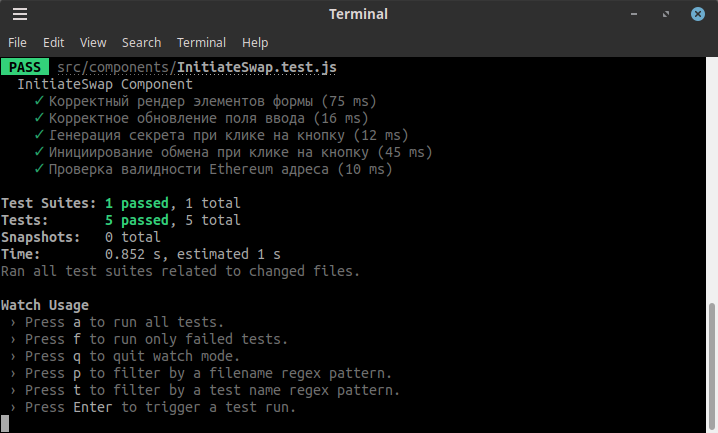
\includegraphics[scale=0.65]{res/console-out}
\caption{Вывод консоли после запуска тестов}
\label{pic:InitiateSwapTestConsole}
\end{figure}

Представленные тесты обеспечивают частичную проверку некоторых функций компонента \textit{InitiateSwap}, включая рендеринг, обработку пользовательского ввода и взаимодействие с внешними библиотеками. В действительности для тестирования сервиса было разработано множество тестов, но приводить их все в данном отчёте не целесообразно.

\subsection{Системное тестирование}

Системное тестирование связано с рядом сложностей, основная из которых это подготовка тестового окружения.

\subsubsection{Разворачивание тестовой сети Ethereum}

Для локальной разработки и тестирования Ethereum широко используется фреймворк Ganache. Это инструмент для запуска сети Ethereum на тестовом стенде, который позволяет разработчикам создавать, тестировать и развертывать смарт-контракты в безопасной и контролируемой среде. Ganache обладает полезными качествами, необходимыми разработчику:

\begin{enumerate}

\item Локальная сеть Ethereum.\\
Ganache запускает локальную версию сети Ethereum, позволяя вам разворачивать и тестировать смарт-контракты без необходимости взаимодействия с основной сетью (mainnet) или тестовыми сетями (testnet).

\item Контроль над сетью.\\
Разработчик может контролировать параметры сети, такие как число генерируемых блоков, сложность майнинга, учетные записи и их баланс. Это позволяет моделировать различные сценарии и тестировать поведение смарт-контрактов в разных условиях.

\item Легкий доступ к аккаунтам.\\
Ganache предоставляет готовые учетные записи с предустановленным балансом ETH, что упрощает процесс разработки и тестирования.

\item UI интерфейс и командная строка.\\
Ganache доступен как в виде графического интерфейса (Ganache UI), так и в виде утилиты командной строки (Ganache CLI), что позволяет выбрать наиболее удобный способ работы.

\end{enumerate}

Можно произвести запуск Ganache в Docker контейнере, для этого используем следующую команду для запуска:

\begin{lstlisting}[style=CommandLineStyle, belowskip=-2 \baselineskip]
$ docker run -d -p 8545:8545 --name ganache trufflesuite/ganache --accounts 10 --defaultBalanceEther 100
\end{lstlisting}
\vspace{-10pt}

Этой командой мы запутили тестовую сеть Ethereum, которая доступна на порту 8545, а так же создали 10 аккаунтов, с балансом в 10 монет у каждого.

Чтобы увидеть аккаунты, их баланс и другие параметры сети можно выполнить следующую команду 

\begin{lstlisting}[style=CommandLineStyle, belowskip=-2 \baselineskip]
$ docker logs ganache
\end{lstlisting}

Примерый вывод этой команды представлен в листинге \ref{lst:ganachelog}. 

\lstinputlisting[language={}, caption={Список доступных аккаунтов в тестовой сети Ethereum}, captionpos=t, label=lst:ganachelog]
{res/ganachelog.txt}

Теперь мы можем развертывать и тестировать смарт-контракты в локальной сети Ethereum, запущенной с помощью Ganache.

\subsubsection{Деплой смарт-контракта в тествую сеть Ethereum}

Для подулючения к тестовой сети можно использовать Truffle или сразу Web3.js.

Новый проект миграции можно подготовить командой

\begin{lstlisting}[style=CommandLineStyle, belowskip=-2 \baselineskip]
$ truffle init
\end{lstlisting}

Сприпт миграции представлен в листинге \ref{lst:TruffleDeploy}. Он полагается на то, что файл смарт-контра доступен по пути \textit{contracts\\HTLCContract.sol}.

\lstinputlisting[language=JavaScript, caption={Скрипт миграции Truffle}, captionpos=t, label=lst:TruffleDeploy]
{res/contract_deploy.js}

Для подключения к тестовой сети, нужно указать её адрес и порт, как это показано в листинге  \ref{lst:TruffleConnect}. Там же показан и выбор версии компилятора Splidity.

\lstinputlisting[language=JavaScript, caption={Подключение к тестовой сети}, captionpos=t, label=lst:TruffleConnect]
{res/truffle-config.js}

Провести развёртывание контракта можно командной
\begin{lstlisting}[style=CommandLineStyle, belowskip=-2 \baselineskip]
$ truffle migrate
\end{lstlisting}

Эта команда скомпилирует смарт-контракт и развернет его на указанной в конфигурации сети. Теперь смарт-контракт развернут на Ganache и готов к тестированию и дальнейшему взаимодействию.

\subsubsection{Разворачивание тестовой сети BitShares}

Подготовка и запуск тестовой сети Bitshares так же возможна через Docker. Для этого можно выполнить следующую команду

\begin{lstlisting}[style=CommandLineStyle, belowskip=-2 \baselineskip]
$ docker run -d -p 8090:8090 -p 8091:8091 -v $(pwd)/bitshares_data:/bitshares/witness_node_data_dir --name bitshares-testnet bitshares/bitshares-core:latest
\end{lstlisting}

Эта команда создаст и запустит Docker контейнер в фоновом режиме. Порты 8090 и 8091 проброшены для доступа к PRC и P2З интерфейсам. Локальная директория bitshares\_data смонтирована в контейнер для хранения данных блокчейна.

После этого нужно подлкючиться к ноде используя CLI-кошелёк и выполнить следующие три команды

\begin{lstlisting}[style=CommandLineStyle, belowskip=-2 \baselineskip]
> import_key nathan "5KQwrPbwdL6PhXujxW37FSSQZ1JiwsST4cqQzDeyXtP79zkvFD3"
> import_balance nathan ["5KQwrPbwdL6PhXujxW37FSSQZ1JiwsST4cqQzDeyXtP79zkvFD3"] true
> upgrade_account nathan true
\end{lstlisting}

Первая команда позволяет импортировать приватный ключ пользователя nathan. Вторая команда инициирует перевод средств, заложенных в генезисе, на счёт пользователя, и далее он может распоряжаться этими средствами. Последняя команда переводит пользователя в расширенный режим, где ему открываются дополнительные возможности по управлению сетью.

\subsubsection{Проведение атомарного свопа в тестовых сетях}

Интерфейс сервиса осуществления атомарных свопов между Ethereum (ETH) и BitShares (BTS) представлен на рис. \ref{pic:ServiceInterface}. Сразу под заголовком находится выбор вкладок: одна отвечает за работу с  Ethereum, а другая вкладка для выбора BitShares.

\begin{figure}[H]
\centering
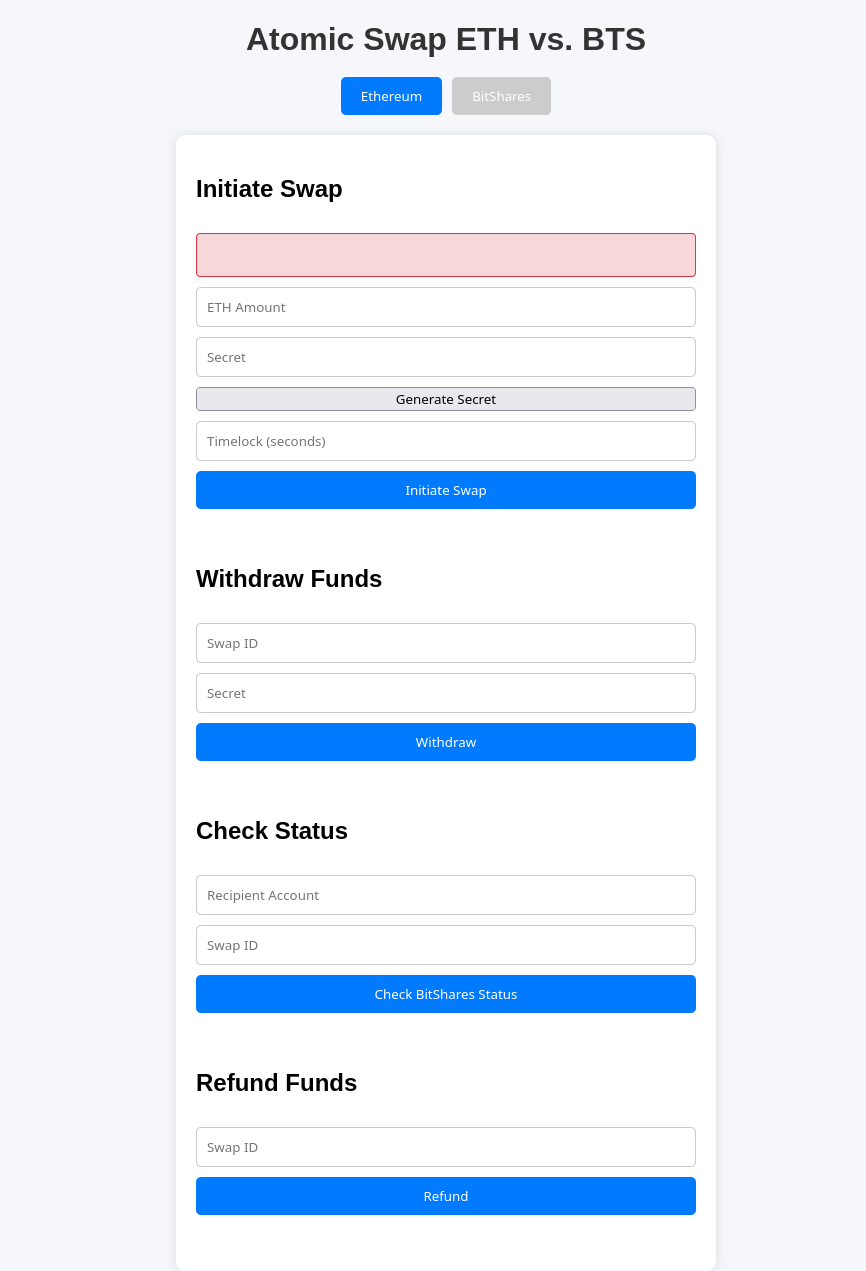
\includegraphics[scale=0.4]{res/ServiceInterface}
\caption{Пользовательский интерфейс сервиса обмена}
\label{pic:ServiceInterface}
\end{figure}

Основная часть интерфейса разделена на четыре секции:
\begin{itemize}
\item Первая секция называется "Initiate Swap". В этой секции пользователь может ввести сумму ETH, секрет, и время блокировки в секундах. Форма реагирует на ввод адреса получателя, проверяя что он является валидным адресом сети Ethernet. Адрес отправителя не нужен, т.к. он будет получен из подписи транзакции. Пользователь может самостоятельно задать секрет, либо сгенерировать его случайным образом. Для генерации случайного секрета предусмотрена отдельная серая кнопка "Generate Secret". Для завершения процесса инициации свопа имеется синяя кнопка "Initiate Swap".

\item Вторая секция называется "Withdraw Funds". Здесь пользователь может ввести идентификатор свопа (Swap ID) и секрет, после чего нажать синюю кнопку "Withdraw" для вывода средств на свой кошелёк. Как и в прошлом случае, адрес кошелька нам не нужен, мы получим его из подписи.

\item Третья секция, "Check Status", позволяет пользователю проверить статус свопа в сети BitShares. Для этого необходимо ввести учетную запись получателя и идентификатор свопа, а затем нажать синюю кнопку "Check BitShares Status". В данном случае, у нас нет возможности получить что либо из подписи, т.к. речь идёт о совершенно другом блокчейне, со своими структурами данных.

\item Четвертая и последняя секция называется "Refund Funds". В этой секции пользователь может ввести идентификатор свопа и нажать синюю кнопку "Refund" для возврата средств. Средства будут возвращены в случае, если они не были востребованы получателем, а срок действия контракта уже вышел. В случае с BitShares такой кнопки нет, т.к. там средства возвращаются отправителю автоматически.
\end{itemize}

Интерфейс предоставляет пользователю необходимый минимум инструментов для инициации атомарного свопа, вывода средств, проверки статуса транзакции и возврата средств в случае необходимости.

На рис. \ref{pic:ChromMetamask} изображен процесс подписания транзакции средствами MetaMask в браузере Chrome. Секция "Initiate Swap" заполнена тестовыми данными, и тут следует обратить внимание на поле с адесом получателя. Сервис воспринял строку "0xc0ffee254729296a45a3885639AC7E10F9d54979" как валидный ETH адрес, в результате поле ввода подкрашено зелёным цветом. Справа от основного интерфейса отображается всплывающее окно MetaMask. В этом окне заголовок "Connect with MetaMask" предлагает пользователю выбрать аккаунт для использования на данном сайте. Отображен аккаунт "Account 1 (0x5d7c3...eab8b)" с балансом 0 ETH. Этот аккаунт выбран для подключения, что отмечено галочкой. В верхней части этого окна виден адрес подключения http://127.0.0.1:3000, что говорит о тестовой сети.

\begin{figure}[H]
\centering
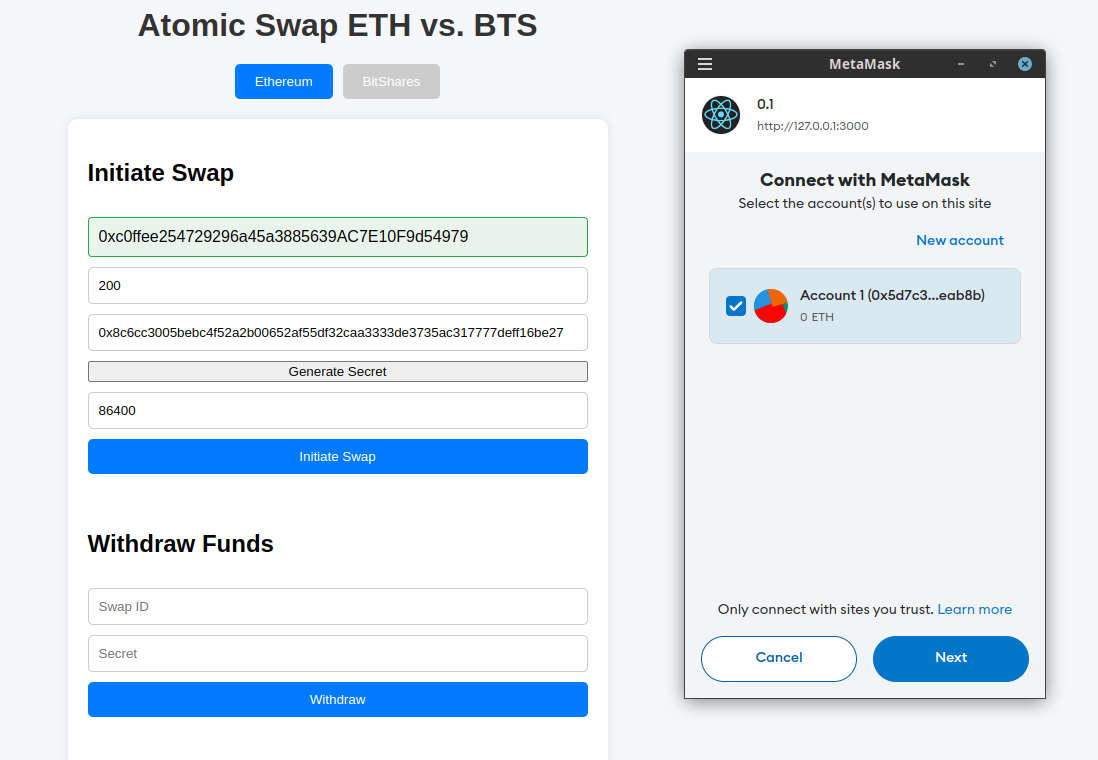
\includegraphics[scale=0.4]{res/ChromMetamask}
\caption{Браузер Chromium и криптокошелёк Metamask}
\label{pic:ChromMetamask}
\end{figure}

На рис. \ref{pic:FFEnkrtpt} так же изображен процесс подписания транзакции, только на этот раз используется браузер FireFox и окно авторизации Enkrypt (MyEtherWallet). Адрес получателя "0xc0ffee254729296a45a3885639AC7E10F9d54979" распознан как валидный, поэтому подсвечен зелёным. Интерфейс предупреждает пользователя, что его действия раскроют публичный адрес, баланс кошелька и активность для сети "127.0.0.1", которая является тестовой площадкой.

\begin{figure}[H]
\centering
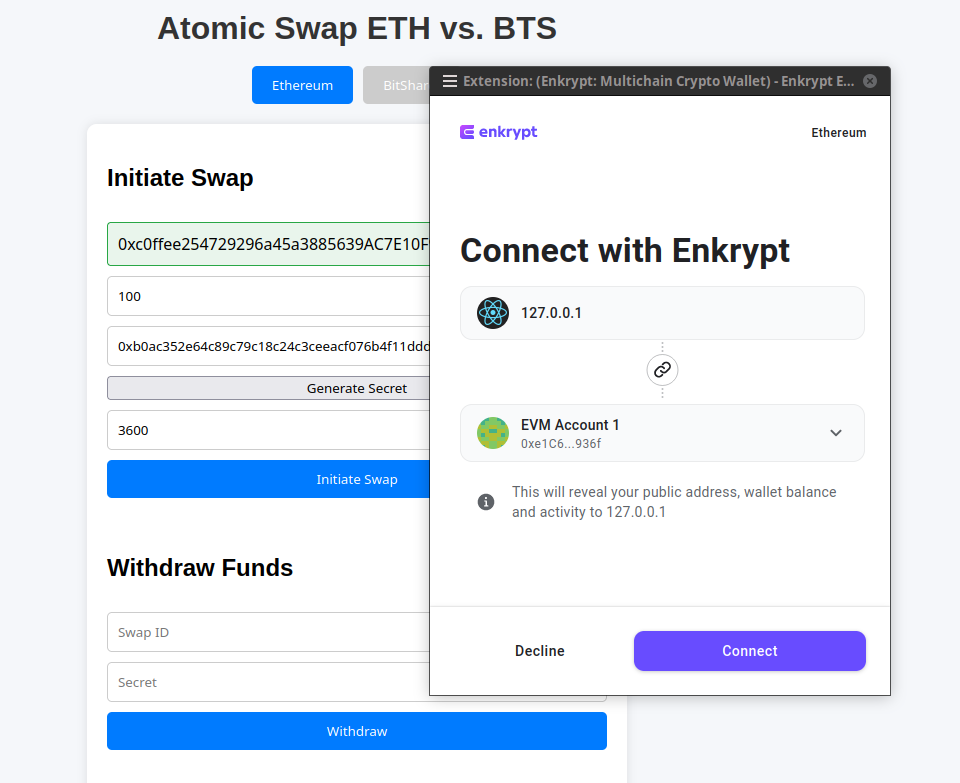
\includegraphics[scale=0.4]{res/FFEnkrtpt}
\caption{Браузер FireFix и криптокошелёк Enkrtpt (MyEtherWallet)}
\label{pic:FFEnkrtpt}
\end{figure}

Когда все контракты выполнены, баланс пользователя изменяется в криптокошельках. В этом контексте, криптокошельки не являются частью сервиса, поэтому их изображение тут не приводится. Сервис не знает баланс пользователя, хотя технически такую возможность реализовать можно.

Проводить операции с Ethereum достаточно просто. В случае с Bitshares, пользователю нужно использовать CLI-кошелёк и самостоятельно заботиться о безопасности своего приватного кошелька. Очевидно, это достаточно неудобно для конечных пользователей. Поддержки BitShares со стороны основных криптокошельков на данный момент нет, но это вполне можно реализовать внутри сервиса, если решить задачу надёжного хранения ключа.

Это может стать темой для дальнейших исследований.

\section{Выводы}

Исследование существующих подходов к межсетевому обмену, таких как использование доверительных сторон, мостов и пулов ликвидности, выявило ряд существенных недостатков. Метод атомарных свапов с использованием HTLC признан наиболее эффективным и безопасным решением для межсетевого обмена. Отсутствие централизованных элементов, гарантированная безопасность, фиксированная цена и возможность адаптации существующих блокчейнов делают этот подход оптимальным для построения сервиса обмена активами.

В этом разделе мы описали структуру сервиса, алгоритм его работы и выбор технологий для разработки. В качестве основного инструмента для построения пользовательского интерфейса был выбран React. Выбор Ethereum обусловлен наличием развитой инфраструктуры для создания и выполнения смарт-контрактов, а BitShares - высокой производительностью и низкими комиссиями за транзакции.

В разработке прототипа сервиса были решены следующие задачи:
\begin{itemize}
\item Создан веб-интерфейс на React, обеспечивающий удобное управление процессом обмена активами.
\item Разработан смарт-контракт для Ethereum, реализующий механизм HTLC.
\item Обеспечено взаимодействие сервиса с API блокчейна BitShares для управления HTLC-контрактами.
\end{itemize}

Представленное решение гарантирует полую децентрализация сервиса, исключающая необходимость доверия между сторонами сделки или к третьим сторонам.

В конце раздела, описывается процесс модульного и системного тестирования. Модульные тесты покрывают функциональность отдельных компонентов сервиса, а системное тестирование проводилось в тестовой сети Ethereum с использованием Ganache и в тестовой сети BitShares. Так же отмечены некоторые минусы, связанные с удобством пользователя, устранение которых может стать темой дальнейших исследований.
